\documentclass[11pt, aspectratio=169, modernfonts]{beamer}
%-----------------------------------------------------------------------
% LaTeX packages
%-----------------------------------------------------------------------
\usepackage{amsfonts}
\usepackage{amsmath}
\usepackage{amsthm}
\usepackage{tabto}
\usepackage{booktabs}
\usepackage{hyperref}
\usepackage{xspace}
\usepackage[utf8]{inputenc}
\usepackage{fancyvrb}
\usepackage{stmaryrd}
\usepackage{caption}
%\usepackage{subcaption}
\usepackage{listings}
\usepackage{pifont}
\usepackage{multicol}
\usepackage{placeins}
\usepackage{verbatim}
\usepackage{wrapfig}
\usepackage{subfig}
\usepackage{minted}
\usepackage[english]{babel}
%\usepackage[a4paper,left=2cm,right=3cm,top=2cm,bottom=2cm]{geometry}

%-----------------------------------------------------------------------
% Theorems
%-----------------------------------------------------------------------
\usepackage{pgf}
\usepackage{tikz}
\usetikzlibrary{arrows,automata}
\usepackage{graphicx}
\usepackage{setspace}
\usepackage{float}
\usepackage{amssymb}
\usepackage{mathtools}
\usepackage{tabto}
\usepackage[T1]{fontenc}
\usepackage{xcolor}
\newtheorem{thm}{Theorem}[section]
\newtheorem{cor}[thm]{Corollary}
\newtheorem{lem}[thm]{Lemma}
\newtheorem{prop}[thm]{Proposition}
\theoremstyle{definition}
\newtheorem{defn}[thm]{Definition}
\theoremstyle{remark}
\newtheorem{rem}[thm]{Remark}

% Alternative theme
%-----------------------------------------------------------------------
%\usetheme[progressbar=frametitle]{metropolis}
%\DeclarePairedDelimiter\ceil{\lceil}{\rceil}
%\DeclarePairedDelimiter\floor{\lfloor}{\rfloor}

\usetheme{CambridgeUS}
\definecolor{midnightblue}{rgb}{0,.25,.5}
\definecolor{darkblue}{rgb} {0.125,0.25, 0.625}
\definecolor{darkgreen}{rgb}{0.125,0.625,0.25}
%\definecolor{darkred}{rgb}  {0.625,0.125,0.25}
\definecolor{darkred}{rgb}  {0.0,0.4,0.59}

\mode<presentation>
{
  \useinnertheme{rectangles}
  \setbeamertemplate{navigation symbols}{}
}

\setbeamercolor{footlinecolorl}{fg=black,bg=lightgray}
\setbeamercolor{footlinecolor}{fg=black,bg=gray}
\setbeamercolor{footlinecolord}{fg=black,bg=darkgray}
\setbeamercolor{block title}{bg=darkred,fg=white}

\setbeamertemplate{itemize item}{\color{darkred}$\blacksquare$}
\setbeamertemplate{itemize subitem}{\color{darkred}$\blacktriangleright$}
\setbeamercolor{item projected}{bg=darkred}
\setbeamertemplate{enumerate items}[default]
\setbeamercolor{enumerate item}{fg=darkred}
\setbeamercolor{enumerate subitem}{fg=darkred}
\setbeamercolor{enumerate subsubitem}{fg=darkred}
\definecolor{rulec}{RGB}{235,129,27}
%-----------------------------------------------------------------------
% Macros
%-----------------------------------------------------------------------
\newcommand{\eg}{e.g.,\xspace}
\newcommand{\encrypt}[1]{\ensuremath{E(#1)}\xspace}
\newcommand{\decrypt}[1]{\ensuremath{D(#1)}\xspace}
%-----------------------------------------------------------------------
\usepackage[utf8]{inputenc}
\usepackage{csquotes}
\usepackage{biblatex}

% ---------------------------------------------------------------------
% Preamble
% ---------------------------------------------------------------------

\setbeamertemplate{footline}{%
\hbox{%
\begin{beamercolorbox}[wd=.40\paperwidth,ht=4.25ex,left,leftskip=3ex]{author in head/foot}%
    \vbox to4.25ex{\vfil\hbox{\usebeamerfont{author in head/foot} \insertframenumber{} / \inserttotalframenumber \hspace{0.5cm}\insertshortauthor}\vfil}%
\end{beamercolorbox}%
\begin{beamercolorbox}[wd=.30\paperwidth,ht=4.25ex,center]{title in head/foot}%
    \vbox to4.25ex{\vfil\hbox{\usebeamerfont{date in head/foot}Algorithm Engineering}\vfil}%
\end{beamercolorbox}%
\begin{beamercolorbox}[wd=.30\paperwidth,ht=4.25ex,right,rightskip=3ex]{date in head/foot}%
    \vbox to4.25ex{\vfil\hbox{\insertshortdate{}}\vfil}%
\end{beamercolorbox}}%
}

\setbeamertemplate{bibliography item}{\insertbiblabel}

\addbibresource{source.bib}

% ---------------------------------------------------------------------
% Title
% ---------------------------------------------------------------------

\title{Virtualization on x86 Architecture}
\author{Jacob Lammert\and Vladimir Spassov}
\date{04.11.2021}
\institute{Bauhaus-Universität Weimar}

% ---------------------------------------------------------------------

\begin{document}

% listings package, set language
% ---------------------------------------------------------------------
\lstset{language=C}
% ---------------------------------------------------------------------
% Content
% ---------------------------------------------------------------------
\maketitle
%\begin{frame}{}
%     \begin{centering}
%    \begin{beamercolorbox}[sep=8pt,center]{institute}
%      \usebeamerfont{institute}\insertinstitute
%    \end{beamercolorbox}
%    \begin{beamercolorbox}[sep=8pt,center]{title}
%      \usebeamerfont{title}\inserttitle\\
%      \textcolor{rulec}{\rule{0.9\textwidth}{0.5pt}}
%    \end{beamercolorbox}
%    \begin{beamercolorbox}[sep=8pt,center]{date}
%      \usebeamerfont{date}\insertdate
%    \end{beamercolorbox}
%    \begin{beamercolorbox}[sep=8pt,center]{author}
%      \usebeamerfont{author}\insertauthor
%    \end{beamercolorbox}
%\footnotesize
%\makebox[\textwidth][c]{Erstgutachter: PD Dr. Andreas Jakoby}
%\makebox[\textwidth][c]{Zweitgutachter: Prof. Dr. Stefan Lucks}
%  \end{centering}
%\end{frame}

\nocite{*}


% https://www.intel.com/content/www/us/en/products/docs/processors/core/core-technical-resources.html

\begin{frame}{Contents}
    \tableofcontents
\end{frame}

\section{Introduction}

\begin{frame}{Introduction}
    \subsection{Processors at our disposal}
    \begin{figure}
        \centering
        \begin{tabular}{|c|c|c|c|}
        \hline
            CPU Name & total cores & VT-x & base frequency \\
            \hline
            Intel$^{\text{\textregistered}}$ Core\texttrademark\ 2 Quad Q8400 & 4 & yes & 2,66 Ghz\\
            \hline
            Intel$^{\text{\textregistered}}$ Pentium $^{\text{\textregistered}}$ 4 & 1 & no & 2,6 Ghz\\
            \hline
            Intel$^{\text{\textregistered}}$ Core\texttrademark i5-10500 & 6 & yes (with EPT) & 3,1 Ghz\\
            \hline
        \end{tabular}
        \caption{\textbf{Processors at our disposal}}
        \label{fig:processor_overview}
    \end{figure}
\end{frame}

\begin{frame}{Introduction}
    \subsection{IA\_32 System Architecture Overview}
    \begin{figure}
        \centering
        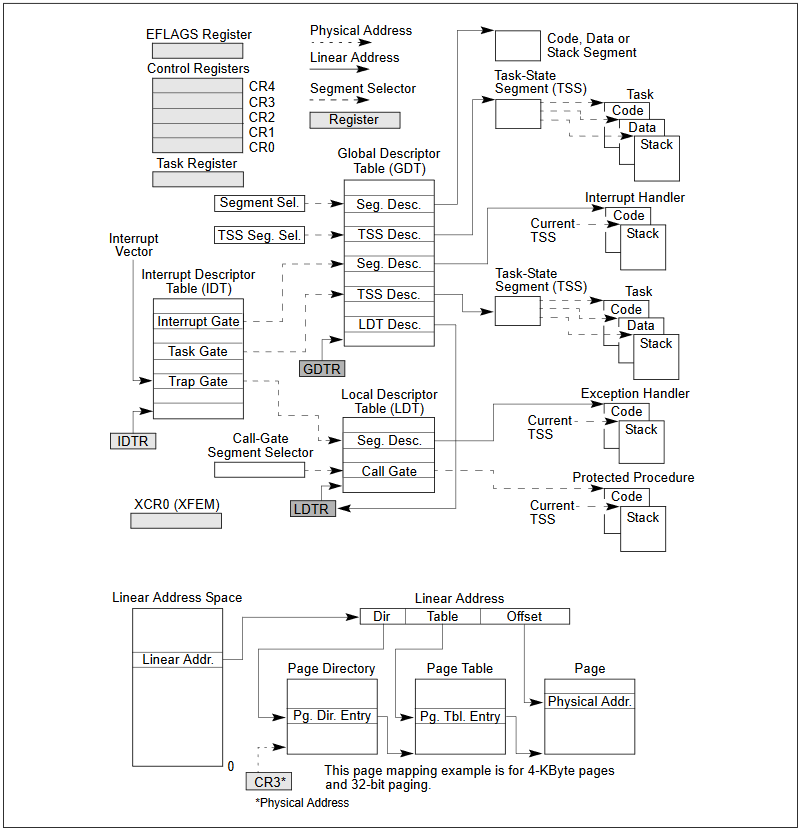
\includegraphics[scale=0.2]{graphics/IA32_architecture.png}
        \caption{IA\_32 System Architecture \cite{architecture64_sof_dev_manuel_vol_3}}
        \label{fig:IA_32_system_architecture}
    \end{figure}
\end{frame}

\begin{frame}{Introduction}
    \subsection{Processor Modes}
    \begin{figure}
        \centering
        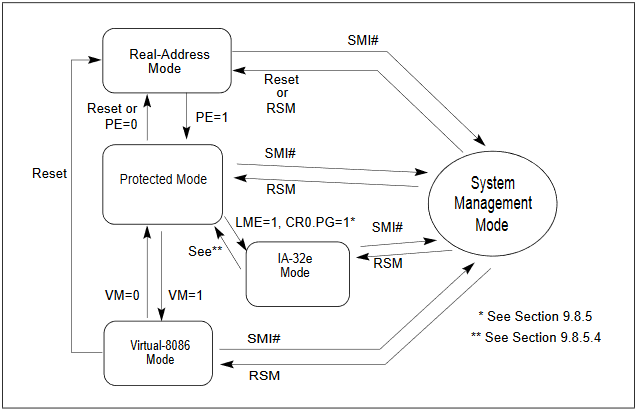
\includegraphics[scale=0.56]{graphics/ProcessorModes.PNG}
        \caption{Processor Modes \cite{architecture64_sof_dev_manuel_vol_3}}
        \label{fig:processor_modes}
    \end{figure}
\end{frame}

\begin{frame}{Introduction}
    \subsection{Hierarchy of Right}
    \begin{figure}
        \centering
        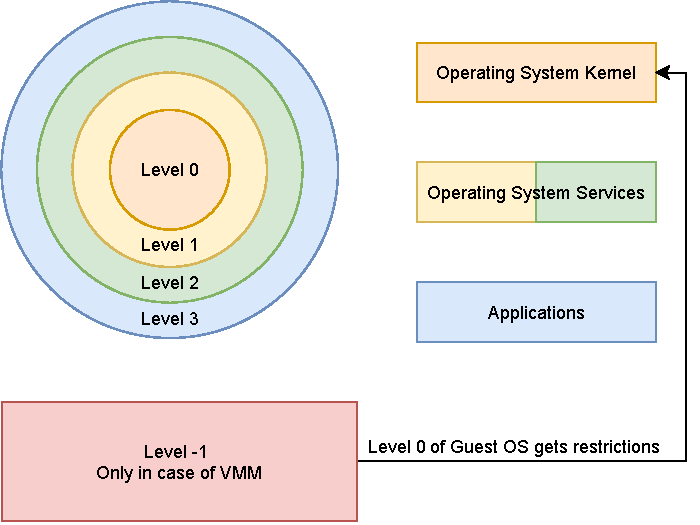
\includegraphics[scale=0.65]{graphics/hierarchyx86.pdf}
        \caption{Hierarchy of Rights}
        \label{fig:x86_hierarchy}
    \end{figure}
\end{frame}

\begin{frame}{x86 VMX \cite{architecture64_sof_dev_manuel_vol_3}}
    \section{x86 VMX}
    \begin{itemize}
        \item basics of virtual machine architecture
        \item overview of the virtual-machine extensions(VMX)
    \end{itemize}
\end{frame}


\begin{frame}{x86 VMX (basics) \cite{architecture64_sof_dev_manuel_vol_3}}
    \subsection{Basics}
    \textbf{Virtual-machine monitors (VMM):}
    \begin{itemize}
            \item host with full control of the processor
            \item A VMM presents guest software with an abstraction of a virtual processor and allows it to execute directly on a logical processor. 
            \item can retain selective control of processor resources, physical memory, interrupt management, and I/O.
    \end{itemize}
    \textbf{Guest software:}
    \begin{itemize}
            \item virtual machines can run independently on the same hardware
            \item the guest software runs with a lower privilege than the VMM (VMM keeps control over certain platform resources)
    \end{itemize}
\end{frame}

\begin{frame}{x86 VMX (instructions)
\cite{architecture64_sof_dev_manuel_vol_3}}
    \subsection{VMX Instructions}
    \textbf{VMX operations}
    \begin{itemize}
        \item VMX root operation - standard for VMM
        \item VMX non root operation - standard for guest software
    \end{itemize}
    \textbf{VMX transitions - transition between VMX non-root and VMX root  operation}
    \begin{itemize}
        \item VM entries - from root to non-root
        \item VM exits - from non-root to root
    \end{itemize}
\end{frame}

\begin{frame}{x86 VMX (instructions)
\cite{architecture64_sof_dev_manuel_vol_3}}
    \begin{figure}
        \centering
        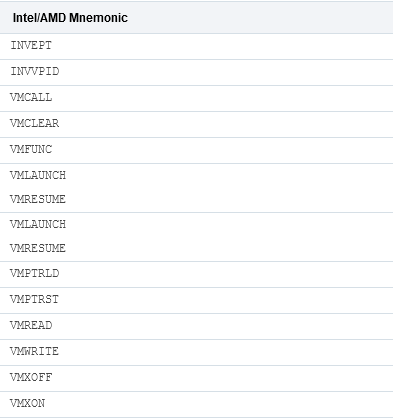
\includegraphics[scale=0.4]{graphics/VMX_instructions.png}
        \caption{Basic VMX instructions \cite{vmx_instructions_oracle}}
        \label{fig:vmx_instructions}
    \end{figure}
\end{frame}

\begin{frame}{x86 VMX (rights)}
    \subsection{VMX Right Levels}
    \begin{block}{VMX root}
        \begin{itemize}
            \item New instructions (all VMX instructions) available.
            \item Certain other registers get limited.
        \end{itemize}
    \end{block}
    \begin{block}{VMX non-root}
        \begin{itemize}
            \item certain instructions (including the new VMCALL instruction) and events cause VM exits
            \item functionality of software in VMX non-root operation is limited
            \item only VMM keeps control of real resources
            \item No bit visible to software indicating that the processor is in VMX non-root operation
        \end{itemize}
    \end{block}
\end{frame}

\begin{frame}{x86 VMX (life cycle)
\cite{architecture64_sof_dev_manuel_vol_3}}
    \subsection{VMX Life Cycle}
    \begin{figure}
        \centering
        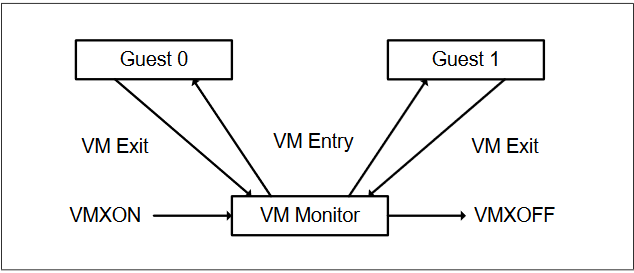
\includegraphics[scale = 0.6]{graphics/vmx_life_cycle.png}
        \caption{Interaction of a Virtual-Machine Monitor and Guests \cite{architecture64_sof_dev_manuel_vol_3}}
        \label{fig:vmx_life_cycle}
    \end{figure}
\end{frame}

\begin{frame}{x86 VMX (life cycle)
\cite{architecture64_sof_dev_manuel_vol_3}}
    \begin{enumerate}
        \item Software enters VMX operation with VMXON instruction
        \item with VMLAUNCH and VMRESUME the VMM effects the VM entry, with VM exit the VMM regains control 
        \item VMM can take action appropriate to the cause of the VM exit end return to the VM with VM entry
        \item with VMXOFF the VMM shuts itself down and leaves VMX operation
    \end{enumerate}
\end{frame}


\begin{frame}{x86 VMX (importent bits)
\cite{architecture64_sof_dev_manuel_vol_3}}
    \subsection{Importent Bits}
    \begin{itemize}
        \item CR4.VMXE[bit 13] must be 1 for execution of VMXON.
        \item CR4.VMXE can not be cleared in VMX operation.
        \item Probably? also 12 Bit of IA32\_EFER\_MSR (Extended Feature Enable Register)
        \item IA32\_EFER\_MSR available only in IA32e mode
    \end{itemize}
\end{frame}

\begin{frame}{x86 VMX (important bits)}
    \begin{figure}
        \centering
        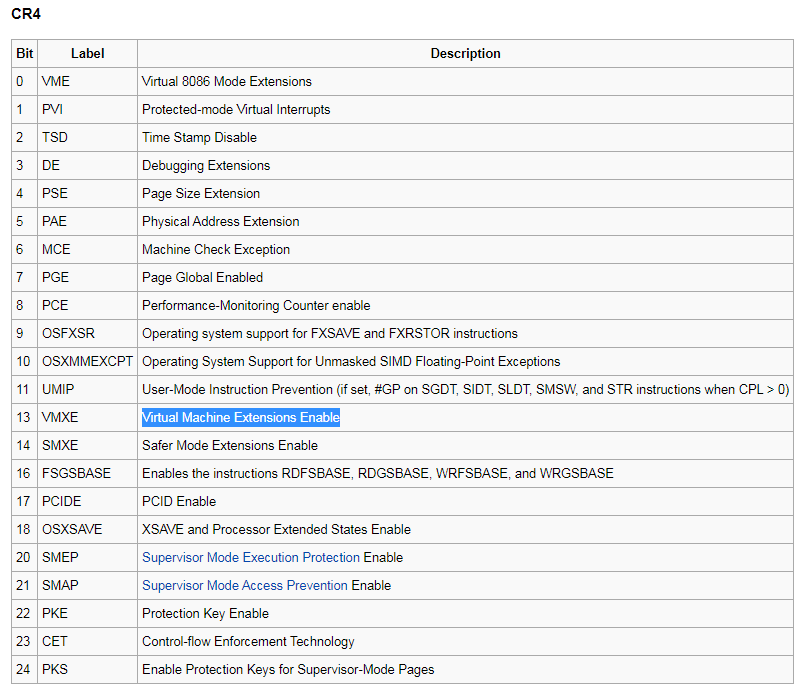
\includegraphics[scale = 0.33]{graphics/CR4.PNG}
        \caption{Control Register 4\cite{cr4}}
        \label{fig:my_label}
    \end{figure}
\end{frame}

\begin{frame}{Recommendations for the Project}
    \section{Recommendations for the Project}
    \begin{block}{Our Problems}
        \begin{itemize}
        \item University does not provide modules for OS development, Assembler etc.
        \item Learning ourselves is possible, but a certain amount of time and effort will be needed
        \item we do not have that much time in our project
    \end{itemize}
    \end{block}
\end{frame}

\begin{frame}{Recommendations for the Project}
    \begin{enumerate}
        \item Formulating final product as specific as possible (concept, sub-goals)
        \item Determine needed Skills (OS dev, IP/TCP Protocol writing, C etc.)
        \item Forming Groups for learning necessary skills
        \item Learn Skills
        \item Implement one sub-goal bye one
        \item Sub-Goals we do not manage to achieve can be shoved into next project (BlueP II or so)
    \end{enumerate}
    \begin{block}{Why?}
        \begin{itemize}
            \item Because necessary knowledge is very very complex 
            \item Minimisation of knowledge we need to acquire in one step will be important
        \end{itemize}
    \end{block}
\end{frame}

\begin{frame}[allowframebreaks]{Quellen}
    \printbibliography
\end{frame}

% ---------------------------------------------------------------------
% Appendix
% ---------------------------------------------------------------------


\end{document}
